\chapter{全局人体特征和局部位置特征的融合增强方法}

在上一章节中,本文通过基准数据集构建方案得到了五种优势互补的多维度合成图像序列,用以实现具有高可控的人体多维度合成图像序列 $I_{1:N}$。在本章中,基于 StyleUNet\cite{styleAvatar} 条件式对抗生成架构,将基准模型从单一条件图像引导的面部重演任务拓展到由多维度合成图像序列引导的带有身体姿态和面部表情的数字人生成任务中。

在该架构下,模型的生成器骨干网络基于 UNet\cite{U-net} 编解码架构,将编码器中每层的特征与上层编码的特征相连,并通过跳跃连接与对应的解码层相连,能够针对多维度合成图像序列进行高质量的特征融合,使得模型生成对应的数字人图像序列。该架构还通过时序位置编码向量表示各帧人物细节变化,使得模型能够建模不同帧间的细节特征。
模型的判别器部分则用于判断生成图像与真实图像之间的差异,并引导生成器生成更加符合视频人物真实数据域的样本。通过基于对抗生成网络设计的模型架构,能够实现单步的数字人图像生成,兼顾了生成的数字人图像的真实性和生成速度。

针对生成质量,在本章节中分别从优化人物整体形象建模和优化人物细节建模两个角度提高数字人建模效果。基于局部位置增强的判别器设计,着眼于提高数字人建模中建模较为困难的手部、眼睛、嘴部等局部位置的像素细节。而基于人体大模型的损失引导策略,通过引入预训练的人体大模型 Sapiens\cite{khirodkar2025sapiens},将生成图像与真实图像的特征差异作为感知损失引导生成器生成更加符合真实人类感知的样本。

与上一章节中任务定义一致,该模型最终以多维度合成图像序列 $I_{1:N}$ 和额外的多维度特征条件 $F_{1:N}$,模型通过训练的方式建模到真实人物视频帧的映射 $P(Y_{1:N}|I_{1:N},F_{1:N})$。在该章节中,$F_{1:N}$ 由显式定义的逐帧时序编码序列 $t_{1:N}$。在模型建模过程中,通过改良的判别器和优化的感知损失提高逐帧生成质量。

本文所提出的方法,分别在实验室数据集和公开数据集中进行了评估实验,验证了基准模型和模块改进的有效性。

\section{概述}

本节所提出基准模型输入输出与前一章中的定义保持一致,
并额外加入了时序编码 $t$ 用以控制模型输出不同帧之间的人物细节变化,其科学问题定义如下:

\textbf{输入:}用以驱动人物表情及动作的N帧多维度合成图像序列$I_{1:N}=\{I_1, \ldots, I_N\}$,该序列包含:
\begin{itemize}
    \item 手部图像序列 $I^{mano}_{1:N}=\{I^{mano}_{1}, \ldots, I^{mano}_{N}\}$
    \item 身体法线图像序列 $I^{normal}_{1:N}= \{I^{normal}_{1}, \ldots, I^{normal}_{N}\}$
    \item 身体语义图像序列 $I^{semantic}_{1:N}=\{I^{semantic}_{1}, \ldots, I^{semantic}_{N}\}$
    \item 神经语义图像序列 $I^{ccbr}_{1:N}=\{I^{ccbr}_{1}, \ldots, I^{ccbr}_{N}\}$
    \item 眼部注视图像序列 $I^{eye}_{1:N}=\{I^{eye}_{1}, \ldots, I^{eye}_{N}\}$
\end{itemize}

任一合成图像均由空间大小一致的三通道图像构成,即 $x_i \in \mathbb{R}^{H \times W \times 3}$,
其中 H 和 W 分别表示为驱动帧帧的长宽。将以上五种模态在通道维度上进行拼接,
得到 $I_i \in \mathbb{R}^{H \times W \times 15}$;
同时还输入时序编码序列 $t_{1:N}=\{t_1, \ldots, t_N\}$,其中 $t_i \in \mathbb{R}^{64}$用以建模不同帧之间人物细节变化的。

\textbf{输出:}模型根据多维度合成图像序列驱动生成对应数字人图像序列。$N$ 帧的图像序列表示为 $\widetilde{Y}_{1:N}=\{\widetilde{Y}_1, \ldots, \widetilde{Y}_N\}$,其中 $\widetilde{Y}_i \in \mathbb{R}^{{H}\times{W}\times{3}}$,其中 H 和 W 分别为视频帧的长宽。

在 \ref{sec:StyleUNet} 节将详细介绍 StyleUNet 模型的基础架构,
该网络将StyleGAN2\cite{styleGAN2} 与UNet\cite{U-net} 结构相结合,
从而将 StyleGAN2 模型由解码器结构拓展成了 UNet 框架的编解码结构,使得模型从无条件生成拓展成条件对抗生成。此外,模型基于小波变换的设计有效地将模型的空间维度进行了压缩,降低了参数量。

在 \ref{sec:discriminator} 节中将介绍局部位置增强的判别器改进设计,
通过在数字人多个视觉关键位置构建对应的判别器,确保生成器模型生成的样本在局部位置上更符合真实分布映射。

在 \ref{sec:sapiens} 节中将介绍基于人体表征大模型的特征引导策略,用以提升生成器建模数字人的整体质量。

\section{基于对抗生成的主干网络模型}
\label{sec:StyleUNet}
本文的网络架构基于 StyleUNet\cite{styleAvatar} 模型构建,与原始模型相比,
将输入从面部 Faceverse\cite{wang2022faceverse} 渲染图像序列拓展到上文构建的多维度合成图像序列,
其模型整体结构如图~\ref{fig:main}~所示。其中二维离散小波变换单元能够从原始图像中抽取含有空间和频率信息的特征图,并降维图像分辨率,减少模型内部中间卷积层中的运算量。接下来各小节中,将针对模型的各个组成部分进行进一步分析。

\begin{figure}[!htbp]
	\centering
	\includegraphics[width=0.9\textwidth]{./m_figures/chapter4/主图.pdf}
	\caption{StyleUNet 的数字人生成网络架构图}
	\label{fig:main}
\end{figure}

\subsection{时序映射网络和时序编码}

本文希望建模的数字人姿态主要受到来自多维度合成图像序列的控制,使得生成的人物动作和表情与输入的多维度合成图像序列保持一致。
但数字人在建模过程中,还涉及许多与动作控制无关的细节变化,如头发、衣服褶皱,光照变化等等。
因此在 StyleGAN2~\cite{styleGAN2} 噪音映射网络的基础上,引入时序编码 $t$,用以在模型中建模生成图像序列中不同帧之间人物的非动作细节变化。

该时序映射网络与 StyleGAN2 噪音映射网络基本结构一致,如图~\ref{fig:time}~所示。
由逐像素通道归一化(Pixel Normalization)\cite{stylegan}和四层全连接层组成,
其中使用LeakyRelu(LReLU) \cite{lrelu} 作为各层的激活函数。
该网络将时序编码 $t$ 转换为时序风格向量 $\mathcal{W}$,
并通过生成器解码器层中的样式调制将 $\mathcal{W}$ 注入到生成器解码器层中不同层次的特征图中。
与原始噪音映射的思路一致,映射网络通过将 $t$ 与 $\mathcal{W}$ 在映射网络中进行解耦,使 $\mathcal{W}$ 能够更好地控制不同帧之间人物形象的细节差异。

\begin{figure}[!htbp]
	\centering
	\includegraphics[width=0.9\textwidth]{./m_figures/chapter4/时序映射网络.pdf}
	\caption{时序映射网络结构图}
	\label{fig:time}
\end{figure}

针对时序编码 $t$,采用类似 Transformer\cite{transformer} 当中的正余弦位置编码方法对原始时序信息进行编码,通过交替使用不同频率正弦和余弦函数,能够不重复的表征每帧的时序位置信息,如公式(\ref{eq:pos_enc})所示。
\begin{equation}
PE(\phi) = (\phi,\sin(\phi \times 2^0), \cos(\phi \times 2^0), \sin(\phi \times 2^1), \cos(\phi \times 2^1), \ldots, \sin(\phi \times 2^k))
\label{eq:pos_enc}
\end{equation}

其中$\phi$表示输入序列的原始位置标量,$k$ 表示为时序编码向量长度 $\text{length}/2-1$。
具体来说,在 StyleUnet\cite{styleAvatar} 中的位置编码 $\phi$ = $F_i/F_{total}$,
将所有的帧输入视为一整个序列,使用当前帧号 $F_i$ 除以总帧数 $F_{total}$ 作为输入的时序标量。
但在实际实验中发现采用此种位置编码方式,当帧序列过长时,$F_{total}$ 取值较大,在帧数 $F_i$ 较小时,生成视频帧中会产生明显的画面闪烁问题。

因此进一步,本文将输入的帧序列分为若干子序列片段,修改为两段位置编码,分别是当前子序列中视频帧位置编码 $\phi_1 = VF_i/VF_{total} $ 和不同子序列间位置编码 $\phi_2 = V_i/V_{total}$。
最终时序编码表示为 $t = PE(\phi_1) + PE(\phi_2)$。其中 $VF_i$ 和 $VF_{total}$ 分别表示该子序列片段中当前帧号和总帧数,
$V_i$和$V_{total}$表示当前子片段序号和总片段数。后续实验证明,采用该双段时序编码方式,能够很好的克服视频帧闪烁问题。

基于特定数字人进行训练建模以后,存储其建模过程中所使用的时序编码。在实际推理驱动时,使用建模阶段对应的时序编码。

\subsection{生成器模型结构}

生成器部分由逐层的编码器和解码器组成,一共由 $d$ 层组成。以第 $d$ 层为例,编码器单元如图~\ref{fig:encoder}~所示,主要由图像编码层和特征卷积层卷积单元组成。其中$f_{d-1}$和$I_{d-1}$表示上一层的输出特征和输出图像,$f_{d}$ 和 $I_{d}$ 表示当前层的输出特征与图像。

编码器旨在通过降采样得到输入多维度合成图像 $I$ 的多级分辨率特征图。其中图像编码器将来自上一层的 $I_{d-1}$ 进行降采样,在经过卷积变换后和上一层输出的特征图 $f_{d-1}$ 相加。特征卷积层进一步利用卷积神经网络层将图像编码器输出的特征进行降采样和特征抽取,并通过残差连接的方式,将输出的特征 $f_{d}$ 输入到下一编码器单元和对应的解码器单元中。

\begin{figure}[!htbp]
	\centering
    \scalebox{0.75}{
	\includegraphics[width=0.9\textwidth]{./m_figures/chapter4/编码器单元.pdf}
    }
	\caption{编码器结构图}
	\label{fig:encoder}
\end{figure}

解码器旨在利用对应编码层特征 $f$ 和输入的时序风格向量 $\mathcal{W}$ 对生成式数字人形象进行合成,以第 $d$ 层为例,其结构如图~\ref{fig:decoder}~所示。
其中 $\widetilde{Y}_{d-1}$ 表示来自上一层解码器输出的图像,$\widetilde{Y}_{d}$ 表示当前层的解码器输出图像,
$f_0$ 表示来自第 0 层的编码器特征,这是因为在解码器单元与编码器单元成上下对称结构,
因此第 $d$ 层解码器接收来自 0 层的编码器输出特征 $f_0$,以此类推 $d-1$ 层的解码器接收 $f_1$。
解码器中的调制卷积来自于 StyleGAN2\cite{styleGAN2},由线性调制和卷积核归一化组成。
通过调制卷积的方式能够很好的将时序风格向量 $\mathcal{W}$ 应用到输入的特征图权重上。

\begin{figure}[!htbp]
	\centering
	\includegraphics[width=0.9\textwidth]{./m_figures/chapter4/解码器单元.pdf}
	\caption{解码器结构图}
	\label{fig:decoder}
\end{figure}

对于风格卷积层,其主要作用是进一步将对应编码器层的特征与 $\mathcal{W}$ 进行融合,将对应时序帧的人物细节融合到隐式特征表示当中。
而图像解码层将当前层风格卷积层输出的隐式特征表示进一步调制后解码成相应的图像渲染特征信息;通过跳跃连接将来自上一层的 $\widetilde{Y}_{d-1}$ 上采样后与图像渲染特征信息进行相加,而后增加逐通道偏置量 $b_{d}$,最终得到当前层的输出图像 $\widetilde{Y}_{d}$。

此外在本文中,模型建模多维度合成图像域到真实人物图像域的映射。因此,本文参考 StyleGAN3\cite{stylegan3} 中的策略,去除了生成器单元中用以增加多样性的随机高斯噪音层。使得模型输出完全基于由时序编码的风格向量 $t$ 和编码多维度合成图像组产生的逐层次特征。

\subsection{判别器结构}

判别器用于区分模型真实人人物视频帧 $Y$ 和生成人物视频帧 $\widetilde{Y}$,通过对抗学习的方式提高生成器的生成能力。判别器为仅编码器结构,其基本单元与生成器中编码单元一致。通过逐层降采样的方式,对输入图像进行特征提取。最终该编码器输出特征图 $f_{d}$ 。此时计算该特征图中逐像素的标准差,作为额外的特征信息 $f_{std}$。最终判别器通过在通道维度拼接特征图 $f_{d}$ 和 $f_{std}$,利用卷积层和全连接层输出单一判别得分。
% 1.26 晚
在该方法中,判别器模型需要判别对应多维度合成图像输入条件下的人物视频帧图像真假。
因此将多维度合成图像以通道维度拼接的方法,与视频帧图像一起输入到判别器模型当中。
即 $I_{discriminator} = \text{concat}(I,\widetilde{Y})$, 其中concat表示通道维度拼接。

\subsection{模型损失函数}

生成器 $G$ 的损失函数由三部分组成,分别是基于像素重建的 $L1$ 损失,
基于神经网络特征的图像感知损失 $ L_{fet}$,对抗损失$L_{adv}$。
生成器 $G$ 的损失函数如(\ref{eq:loss})所示。
其中 $\lambda_{adv}$,$\lambda_{l1}$,$\lambda_{fet}$ 分别表示对抗损失,$L1$ 损失和感知损失在总损失中的权重系数。
\begin{equation}
    L_G = \lambda_{adv} L_{adv} + \lambda_{l1} L_{1} + \lambda_{fet} L_{fet}
    \label{eq:loss}
\end{equation}

本文生成对抗损失使用 softplus\cite{softplus} 进行约束。
对抗损失 $L_{adv}$ 的计算公式如(\ref{eq:L_G})所示,
其中 $D$ 代表判别器网络,$G$ 代表生成器网络,$I$  和$t$ 分别代表合成图像输入和时序编码输入。
$D(G(I))$ 代表生成样本在判别器中的得分,生成器模型将最大化判别器得分作为目标来优化自身参数。
\begin{equation}
    L_{adv} = log(1+exp(D(G(I,t),I)))
    \label{eq:L_G}
\end{equation}

判别器D的损失函数 $L_D$ 如公式(\ref{eq:L_d})所示,其中 $Y$ 代表真实人物视频帧。判别器通过最大化真实人物视频帧的输出得分,并最小化生成人物视频帧得分进行训练。
\begin{equation}
    L_D = log(1+exp(-D(Y,I)))+log(1+exp(D(G(I,t),I)))
    \label{eq:L_d}
\end{equation}

\section{局部特征融合增强}
\label{sec:discriminator}
在高保真数字人视频建模任务中,手部、面部等区域是使用者重点关注的部分。当画面中这些区域出现扭曲、变形等失真问题,数字人使用者体验会极大下降。而这些子区域相对于数字人整体画面来说,重建区域较小,但运动丰富,细节复杂,对于神经网络建模来说具有很大的挑战。在对抗生成任务当中,判别器负责鉴别生成器产生的样本来推动生成器形成更符合真实视频的分布映射。因此本节当中使用基于图像子区域的多判别器增强结构,以期望提高数字人关键视觉部位的生成质量。

Vid2vid\cite{vid2vid} 中,提出了在图像的子区域上应用一个单独的基于 PatchGAN\cite{patchGAN} 判别器对生成图像进行判别增强的方法。
Vid2vid中将此判别器应用在人物动作重演任务的头部身份保持中。后续该方法在 head2head++ 方法\cite{head2head++}中进一步验证,该判别器设计能够在一定程度上改良嘴型的重建效果。因此本文针对具有身体的数字人任务,分别引入了左右手判别器 $D_{left}$ 和$D_{right}$,针对面部分别引入了眼部判别器 $D_{eye}$ 和嘴型判别器 $D_{mouth}$。
图~\ref{fig:local_dis}~展示了本文使用的局部位置增强的整体设计框架。

\begin{figure}[!htbp]
	\centering
	\includegraphics[width=0.9\textwidth]{./m_figures/chapter4/局部判别器图.pdf}
	\caption{局部位置增强架构图}
	\label{fig:local_dis}
\end{figure}

与基准模型中的主判别器中类似,判别器需要判别对应合成图像条件下的生成图像,因此对每个局部判别器输入拼接后的对应裁剪后子区域多维度合成图像 $I_{crop}$ 和真实人物视频帧 $Y_{crop}$ 或生成人物视频帧 $\widetilde{Y}_{crop}$。
% 即$I_{discriminator} = concate(I_{crop},\widetilde{Y})$。
但与主判别器中不同的是,对于局部图像进行判别时,不使用全部多维度人体合成图像条件,仅使用与该部位相关联的合成图像信息。
具体来说,眼部判别器输入的条件图像为眼部注视图像 $eye_{crop}$;
手部判别器输入的条件图像为手部图像 $mano_{crop}$ 和神经语义图像 $ccbr_{crop}$;
嘴型判别器输入的条件图像为神经语义图像 $ccbr_{crop}$。将上述判别器统称为局部判别器 $D_{lcoal}$,
生成器的局部对抗生成损失 $L_{local}$ 表示 $n$ 个局部判别器输出分数之和,即表示为公式(\ref{eq:local_adv}):
\begin{equation}
 \begin{split}
    L_{local}^G = & \sum^{n}_{i=1} \lambda_{adv}^iL_{adv}^i \\
    L_{adv}^{local} = & (D_{local}(I_{crop},\widetilde{Y}_{crop}) - 1)^2
 \end{split}
 \label{eq:local_adv}
\end{equation}

局部对抗损失中使用均方误差作为约束,生成器网络最大化$D_{local}$的判别得分,使其趋近于1。
相应的,对于每个局部判别器 $D_{local}$,最大化真实人物视频帧判别分数趋近于1,最小化生成人物视频帧判别分数趋近于0。判别损失表示如公式(\ref{eq:local_dis})所示:
\begin{equation}
       L_{local}^D = (1 - D_{local}(I_{crop},\widetilde{Y}_{crop}) )^2 + (D_{local}(I_{crop},Y_{crop}) - 1)^2
    \label{eq:local_dis}
   \end{equation}

局部判别器方法实质上约束了生成器在对抗学习过程中满足主判别器和多个局部判别器联合分布,以此提高生成器在局部位置增强的效果。

最后,为了得到对应的图像裁剪区域,在该部分引入额外的输入项:人体关键点 $K$。通过关键点对需要裁剪的部位进行定位。
该人体关键点基于 SMPLX\cite{smplx} 关节点和 Faceverse\cite{wang2022faceverse} 关键点提取得到。
此处将具体需要应用关键点裁剪的部位称为 CROP。以左手裁剪 $\text{CROP}^{left}_{1:T}$ 为例,对于其中一帧数据,
将基于左手的 21 个关节点坐标均值作为裁剪中心点 $\text{Mean}^{left}_i$,并基于该中心点与其他关键点的距离确认当前帧的最小裁剪长度 $\text{Min}^{left}_i$。
对于一个序列中的数据,通过遍历每帧得到其在该序列中的最小裁剪长度序列 $\text{Min}^{left}_{1:T}$。取其中的最小裁剪长度的最大值 $\text{Max}(\text{min}^{left}_{1:T})$,并按照比例 $\alpha$ 放大,得到最终的子区域裁剪长度,结合裁剪中心点坐标得到实际裁剪区域 $\text{CROP}^{left}_{1:T}$。


\section{基于预训练大模型的人体全局特征融合}
\label{sec:sapiens}
基于神经网络预训练模型提取生成图像和真实图像的特征能有效模拟图像在内容和结构上与人类感知上的相似程度,根据特征差异作为损失函数可以引导生成器生成更符合人类感知的样本,
提高生成图片的整体质量,减少生成的伪影\cite{lpips},因此感知损失是视频和图像生成任务当中常用的损失之一。如在部分数字人头像驱动任务当中,ArcFace 特征\cite{deng2019arcface}被用来提高人物的身份一致性。

在 StyleUNet 基准模型中,采用基于 VGG网络\cite{vgg} 进行感知损失的计算。
该损失函数使用在 ImageNet 数据集\cite{deng2009imagenet}中预训练的 VGG 网络中多层次特征图来捕捉图片的语义信息,通过计算生成图像和真实图像各层次特征差异来衡量图像的相似性。
在 VGG 结构当中,网络自底向下不同的模型层次特征能够捕获不同粒度的图像语义信息,
最底层的网络特征代表了图片边缘等的低层次特征,高层网络特征特征则包含有图像的抽象语义信息,因此损失函数设计如公式(\ref{eq:vgg_loss})所示:
\begin{equation}
    L_{VGG} = \frac{1}{L}\sum_{l \in L} \lambda_l \left\| \phi_l(\hat{I}) - \phi_l(I) \right\|
    \label{eq:vgg_loss}    
\end{equation}

其中, \( L \) 是选择的 VGG 网络层集合。\( \hat{I} \) 是生成数字人图像,\( I \) 是原视频人物图像。\( \phi_l \) 表示 VGG 网络第 \( l \) 层的特征。 \( \| \cdot \| \) 是 L1 范数,表示两张图像在该层特征空间中的距离。\( \lambda_l \) 是第 \( l \) 层的权重系数,通常用于加权不同层的特征贡献。
%sapiens介绍

预训练大模型指的是在大规模数据集上进行预训练的基础模型,能够为下游任务提供丰富的表示学习能力。该类模型往往满足尺度(Scaling)法则。该法则指的是随着模型规模和计算资源的增加,模型的性能会显著提升,甚至于出现非线性能力提升的涌现现象。该类模型利用微调的方式应用到下游特定任务或直接使用预训练模型进行特征提取。

针对数字人生成任务中的感知损失,本文提出使用预训练的 Sapiens \cite{khirodkar2025sapiens} 模型作为参数冻结的特征提取器,对生成图像和真实图像分别提取特征,并计算特征差异作为损失函数引导生成器生成更符合人类感知的样本。

Sapiens 模型基于 ViT 架构\cite{dosovitskiy2021an} 进行设计,专注于人体表征的提取。
其使用 3 亿张 $1024 \times 1024$ 分辨率的人体图像参照 MAE\cite{he2022masked} 掩码重建的方式进行预训练,
因此经过预训练的 ViT 编码器能够从人物图像当中提取高质量的包含有语义和结构信息的人体特征 Token 序列。
图\ref{fig:sapiens} 中显示了Sapiens如何从一张图像中提取对应的特征 Token 序列。

\begin{figure}[htbp]
	\centering
    \scalebox{0.6}{
	\includegraphics[width=0.9\textwidth]{./m_figures/chapter4/sapiens.pdf}
    }
	\caption{Sapiens 特征提取流程图}
	\label{fig:sapiens}
\end{figure}

具体而言,Sapiens 遵循标准 ViT 构建过程,以 $16 \times 16$ 的窗口大小分块原始图像。此时一张 $1024 \times 1024$ 分辨率下的图像可以被分割为 4096 个 Token 块,其中每个 Token $\in \mathbb{R}^{16 \times 16 \times 3}$。每个 Token 被输入模型后,在线性映射层被展平,并被映射到指定的维度大小并与时序编码进行相加。图像 Token 序列经过若干 Transformer 编码器,得到最终的特征 Token 序列。

本文针对 Sapiens 设计的损失函数其公式定义如(\ref{eq:sapien_loss})所示,其计算 Sapiens 输出的所有特征 Token 间的差异。
\begin{equation}
    L_{sapiens} = \frac{1}{T}\sum_{t \in T}  \left\| \phi(\hat{I_t}) - \phi(I_t) \right\|
    \label{eq:sapien_loss}    
\end{equation}

其中, \( T \) 是图像按照 $16 \times 16 $的窗口大小划分的 Token 的集合。\( \hat{I} \) 是生成数字人图像,\( I \) 是原视频人物图像。\( \phi \) 表示 Sapiens 网络的特征输出。 
\( \| \cdot \| \) 是 L1 范数,表示第 $t$ 个 Token 在特征空间中的距离。


\section{模型测评与实验分析}

\subsection{实验目标与配置}

\textbf{1)实验目标}

本章提出基于全局人体特征和局部位置特征的融合增强方法是针对以 StyleUNet\cite{styleAvatar} 为基础的模型进一步优化数字人建模任务生成质量的方法。
在实验部分,本文将加入了局部位置判别器的条件式对抗生成网络作为基准模型,并基于该基准模型进行实验验证。首先在自采集数据集中对模型参数进行消融,该部分主要针对时序编码器优化方案进行实验验证和基于预训练大模型的全局特征引入方案进行权重消融和模块有效性验证。
为了进一步评估本章数字人在不同场景下的建模效果,在 Ted-talk\cite{ted-talk} 和 How2sign\cite{how2sign} 数据集上进行迁移学习实验。

因此本节实验目标主要有以下二点:
\begin{enumerate}
    \item 参数消融并验证时序编码器改进与大模型引导的有效性。
    \item 在不同场景和人物上评估模型建模效果。
\end{enumerate}

围绕上述目标,本文设计了两组实验来对以上目标展开实验,对本节提出方案进行详细的评估。在实验实施时,为了更好的评估数字人模型重建的图像质量,本文在可视化分析时使用热力图作为分析工具。热力图中根据真实图像与生成图像之间像素值的差异程度映射到不同的颜色通道上。通过 APD\cite{head2head++} 计算相应的像素误差,将误差值使用公式(\ref{eq:heatmap})进行误差归一化,其中 $p$ 代表某一像素位置的误差值,$T_{\max}$ 表示误差阈值。

\begin{equation}
    \hat{p}= \frac{\min({p,T_{\max}})}{T_{\max}}
    \label{eq:heatmap}
\end{equation}

热力图中的低温区域、过渡区域和高温区域分别用蓝色、绿色、红色来表征。为此,其某一像素位置的具体的颜色由公式(\ref{eq:heat})结合归一化后的误差值 $\hat{p}$ 进行计算。

\begin{equation}
    \begin{split}
        R &= 255 \cdot \max\left( 0,\ \hat{p}-1 \right) \\
        B &= 255 \cdot \max\left( 0,\ 1 - \hat{p} \right) \\
        G &= 255 - R - B
        \end{split}
    \label{eq:heat}
\end{equation}


\textbf{2)环境配置}

本方案相关的训练和测试工作的硬件环境如表~\ref{tb:hardware_env1}~所示,软件环境如表~\ref{tb:software_env1}~所示。

\begin{table}[!htbp]
    \centering
    \caption{硬件环境配置}
    \label{tb:hardware_env1}
    \scalebox{0.9}{
    \newcolumntype{Y}{>{\centering\arraybackslash}X}
    \begin{tabularx}{\textwidth}{c Y}
    \hline
    \textbf{硬件名称} & \textbf{具体信息}\\
    \hline
    操作系统 & Ubuntu 22.04 LTS\\
	CPU & AMD EPYC 7763 64-Core Processor @ 3.17GHz\\
	GPU & NVIDIA A100-SXM4-80GB Specs $\times$ 8\\
    内存 & 2TB\\
    \hline
    \end{tabularx}
    }
\end{table}

\begin{table}[!htbp]
    \centering
    \caption{软件环境配置}
    \label{tb:software_env1}
    \scalebox{0.9}{
    \newcolumntype{Y}{>{\centering\arraybackslash}X}
    \begin{tabularx}{\textwidth}{c Y}
    \hline
    \textbf{软件名称} & \textbf{版本信息}\\
    \hline
    Python & 3.9\\
	Pytorch & 2.3.1\\
    CUDA & 1.12.1\\
    \hline
    \end{tabularx}
    }
\end{table}

\textbf{3)数据集配置}

本节实验基于第二章构建的基准数据集的子集,总共采用了三个人物形象。
其中本章使用自采集的新闻播报数据集中室外条件下的走动人物形象进行基准模型的测试与训练。

使用一个来自 Ted-talk 数据集\cite{ted-talk}的全身演讲人物形象和一个来自 How2sign 数据集\cite{how2sign}的半身手语人物形象通过迁移学习的方式从已经在自采集数据集中训练好的基准模型中进行微调学习,验证模型的性能指标。表~\ref{tab:dataset1}~展示了数据集的基本使用情况和人物形象。

\begin{table}[htbp]
    \centering
    \caption{数据集配置}
    \label{tab:dataset1}
    \scalebox{0.8}{ % 缩放表格
    \newcolumntype{Y}{>{\centering\arraybackslash}X}
    \begin{tabularx}{\textwidth}{c Y Y Y}
    \hline
    \textbf{人物形象} & \textbf{示例图片}& \textbf{训练集数量(帧)} & \textbf{测试集数量(帧)}  \\
    \hline
    自采集人物 & 
    \begin{minipage}[Y]{0.25\textwidth}
    \centering
    \includegraphics[width=\linewidth]{./m_figures/chapter4/result/spa0.6b/org.png}
    \end{minipage} & 17,500 & 1,000 \\

    ted-talk全身人物&  
    \begin{minipage}[Y]{0.25\textwidth}
    \centering
    \includegraphics[width=\linewidth]{./m_figures/chapter4/result/ted2/org.png}
    \end{minipage} & 2,500 & 500  \\

    how2sign半身人物&    \begin{minipage}[Y]{0.25\textwidth}
        \centering
        \includegraphics[width=\linewidth]{./m_figures/chapter4/result/how2sign/org.png}
        \end{minipage}  & 3,000 & 750   \\
    \hline
    \end{tabularx}
    }
\end{table}

\textbf{4)实验细节}

\textbf{混合精度训练:}为了进一步加快模型训练速度并降低显存占用,本文中探索为模型提供混合精度训练\cite{micikevicius2018mixed}的支持。混合精度技术在前向传播过程中,对于线性层、激活函数、卷积层等不需要高精度的操作使用 16 位浮点数来提高计算效率,而在梯度计算、权重更新等关键操作中保持 32 位浮点数。在梯度反向传播时通过梯度缩放操作放大梯度值避免在使用 16 位浮点数时由于精度限制,梯度值出现数值下溢。

本文的模型主要结构基于 PyTorch \cite{paszke2019pytorch}进行实现,PyTorch 算子中支持直接的自动混合精度操作。但 StyleUNet \cite{styleAvatar} 中继承自 StyleGAN2 模型\cite{styleGAN2}的上采样单元 UpFirDn2d 和激活函数单元 FusedLeakyReLU 均使用 CUDA \cite{kirk2007nvidia}的方法直接实现。为此,该部分通过修改其算子实现,使得调用对应 CUDA 算子时,将对应向量转化为 16 位浮点数表示并使得 CUDA 核计算行为匹配对应数据类型。这通过引入 PyTorch 中的custom\_fwd,custom\_bwd 方法并修改对应 CUDA 算子的 AT\_DISPATCH 方法实现。前者定义了 PyTorch 在混合精度模式下对算子前向传播和反向传播的调用行为,后者则对应CUDA算子自身被不同数据类型调用时的计算行为模式。

本文将模型分别在两种半精度浮点数 float16 和 bfloat16 数据格式中进行了训练测试实验。其对比如表 \ref{tab:ff} 所示。经过验证,float16 会导致训练不稳定,训练过程中出现 NaN 的数值溢出错误。而 bfloat16 混合精度训练时能够与正常全精度 float32 训练结果中损失下降趋势一致,且数值基本接近。因此本文后续均使用 bfloat16 模式的混合精度进行训练。

\begin{table}[htbp]
    \centering
    \caption{浮点数对比(float16, bfloat16, float32)}
    \begin{tabular}{cccc} \hline
    
    \multirow{2}{*}{\textbf{特性}} & \multicolumn{3}{c}{\textbf{数据类型}} \\ \cline{2-4} 
     & \textbf{float16} & \textbf{bfloat16} & \textbf{float32} \\ \toprule
    位宽 & 16位 & 16位 & 32位 \\ 
    指数范围 & $[-14, 15]$ & $[-126, 127]$ & $[-126, 127]$ \\ 
    符号位 & 1位 & 1位 & 1位 \\
    指数位数 & 5位 & 8位 & 8位 \\ 
    尾数位数 & 10位 & 7位 & 23位 \\ 
    精度 & 较低 & 较低 & 高 \\ 
    存储需求 & 2字节 & 2字节 & 4字节 \\ \bottomrule
    \end{tabular}
    \label{tab:ff}
    \end{table}

\textbf{归一化对齐:}本文使用的 VGG16\cite{vgg} 和 Sapiens\cite{khirodkar2025sapiens} 预训练网络均使用 ImageNet 数据集\cite{deng2009imagenet}的图像均值和方差归一化模型输入范围。
而本文的模型,则直接将像素数值取值范围从$[0,255]$归一化到$[-1,1]$作为输入输出范围,
因此在使用预训练网络进行感知损失监督时,对模型的输入输出范围逆变换回像素空间后再利用 ImageNet 均值和方差进行归一化对齐。

\textbf{模型超参数设置:}
本文模型在数字人训练过程中均使用2e-3的学习率,单卡训练批次大小为 8。训练过程中,使用 Adam 优化器进行模型优化,使用权重为 0.99 的指数移动平均策略平滑模型参数,并使用 bfloat16 混合精度训练。本文的模型在 $ 1024 \times 1024$ 分辨率上进行训练。针对模型实验中的局部判别器权重和主判别器权重均设置为 1。

最后,对于特征损失,使用 VGG 损失时,选择VGG网络中的 $[2,7,12,21,30]$ 层进行损失计算,并对所有层采用相同的权重,其权重系数 \( \lambda_l \) 设置为1。基于VGG网络的特征损失采用 10 的特征权重$\lambda_{fet}$。针对 Sapines 的特征损失 ,本文实验中主要选择使用参数量为6亿(0.6B)的 Sapiens 预训练模型监督 StyleUNet 的训练。同时为了进一步验证大模型的尺度效应,即验证更大的人体预训练模型提取的特征能够更好的引导模型的生成效果,进一步使用10亿(1B)参数量的模型进行结果比较。

\subsection{模型结构与参数消融实验}
\textbf{1)实验设计}

本实验的重点是针对基准模型的数字人模型结构与参数进行消融实验。
在实验中首先通过可视化结果分析本文优化后的时序位置编码与 StyleUNet\cite{styleAvatar} 方法原始时序编码生成结果的差异。其中在基于时序编码的消融实验中,感知损失采用 VGG 网络进行计算。在时序编码实验中,方案一称为“原始时序编码”方案,使用单一时序编码策略,方案二称为“改良时序编码”方案,采用本文提出的两段式时序编码,分别使用子序列位置编码和序列内位置编码。
接着针对 Sapiens\cite{khirodkar2025sapiens} 作为感知损失进行全局特征融合,通过分析其使用不同权重 $\lambda_{sapiens}$ 的过程中,模型本身$L1$ 损失的变化,确定最优的 Sapiens 权重。
本文针对时序位置编码实验,为了分析不同时序编码的作用,使用训练数据进行可视化。
% 探索Sapiens 所使用的超参数。
在确定使用的模型超参后,本文三个模型方案进行定量对比。
其中方案一称为 “VGG” 方案,即在模型训练的时候采用 VGG 网络进行感知损失计算。方案二称为“Sapiens 0.6B”方案,即使用参数量为6亿(0.6B)的 Sapiens 预训练模型进行感知损失计算。方案三称为“Sapiens 1B”方案,即使用参数量为10亿(1B)的 Sapiens 预训练模型进行感知损失计算。以上方案均在自采集数字人上进行训练和测试,采用APD,MAPD,LPIPS,PSNR,SSIM 和 FVD 作为评估指标,其中APD和MAPD用于直接评估视频帧像素差异,LPIPS,PSNR,SSIM用于评估生成视频中单帧质量,FVD用于评估生成视频的质量和时序连续性。最终验证本文所提出的基于 Sapiens 的特征方案相较于原始 VGG 方案的性能差异。

\begin{figure}[!htbp]
	\centering
	\includegraphics[width=0.9\textwidth]{./m_figures/chapter4/result/时序编码消融.pdf}
	\caption{时序编码修正可视化效果对比}
	\label{fig:time-fix}
\end{figure}

\textbf{2)时序编码结果可视化分析}

为了直观的展示 StyelUNet 时序编码方案与本文改良后的时序编码对模型图像生成的影响,图 \ref{fig:time-fix} 中分别展示了对应的原始视频帧、两种不同时序编码下的生成视频帧和与其对应的不带背景掩码的热力图。图中展示了在总一万七五百帧的训练数据中帧号分别为 3 和 6 的多维度合成图像驱动模型生成结果。图中热力图差异显示了“原始时序编码”方案在帧号极小时产生了不稳定的现象,具体表现为与原始数字人视频帧在背景和身体表面产生了较大的整体亮度差异。而本文“改良时序编码”方案很好的生成与原视频帧接近的数字人物形象,因此本文后续将其作为基准模型的时序编码方案。

\textbf{3)Sapiens感知损失可视化分析}

图 \ref{fig:loss_comparison} 对比了使用 Sapiens 0.6B 模型作为$L_{fet}$时,使用不同损失权重$\lambda_{sapiens}$,模型在训练过程中的 $L1$ 损失变化情况。
其中兰色、粉色、黄色曲线分别代表了权重为10,5,1时的$L1$损失变化曲线。使用$L1$损失分析直接反映生成器在训练过程中的图像重建质量。
在图 \ref{fig:spa5} 中分别对比权重 $\lambda_{sapiens}$ 设置为 1 和 5 时的 $L1$ 损失遵循一致的下降曲线趋势,但当感知权重为 5 时,训练的后期将导致 $L1$ 损失增大。
图 \ref{fig:spa10} 中分别对比权重$\lambda_{sapiens}$设置为 1 和 10 的情况,权重为 10 时,$L1$ 变化幅度很大,实质上表现为$\lambda_{sapiens}$权重过大导致反向传播时梯度过大,破坏了模型的正常收敛。因此本文后续将  $\lambda_{sapiens}$ 设置为 1。

\begin{figure}[!htbp]
    \begin{subfigure}[b]{0.45\textwidth}
        \centering
        \includegraphics[width=\textwidth]{./m_figures/chapter4/result/spa5.png}
        \caption{权重 1 与 5 对比}
        \label{fig:spa5}
    \end{subfigure}
	\hfill
	\begin{subfigure}[b]{0.45\textwidth}
        \centering
        \includegraphics[width=\textwidth]{./m_figures/chapter4/result/spa1.jpg}
        \caption{权重 1 与 10 对比}
        \label{fig:spa10}
    \end{subfigure}
    \caption{不同感知损失$\lambda_{fet}$权重下$l1$损失函数图像对比}
    \label{fig:loss_comparison}
\end{figure}

\textbf{4)感知损失实验结果}

三种感知损失函数方案监督模型训练后,模型在测试集中指标结果如下表~\ref{tab:base_comparison}~所示,其中加粗表示最佳结果,下划线表示排名第二的结果。

\begin{table}[!htbp]
    \centering
    \caption{基准模型性能比较}
    \begin{tabular}{@{}lccccccc@{}}
        \toprule
        \textbf{Model} & \textbf{APD $\downarrow$} & \textbf{MAPD $\downarrow$} & \textbf{LPIPS $\downarrow$} & \textbf{PSNR $\uparrow$} & \textbf{SSIM $\uparrow$} & \textbf{FVD $\downarrow$} \\
        \midrule
        VGG         & 4.15 & 28.53  & \textbf{0.019} & \textbf{31.05} & \textbf{0.971} & 111.51 \\
        Sapiens 0.6B & \underline{3.89} & \underline{26.90}  & 0.025 & 29.64 & 0.968 & \underline{99.94} \\
        Sapiens 1B   & \textbf{3.18} & \textbf{20.38}  & \underline{0.024} & \underline{30.17} & 0.968 & \textbf{82.17} \\
        \bottomrule
    \end{tabular}
    \label{tab:base_comparison}
\end{table}

\textbf{5)感知损失实验实验分析}

表~\ref{tab:base_comparison}~展示了各模型在不同性能指标上的表现。“Sapiens 1B”在 APD 和 MAPD 指标上相较于“VGG”具有显著优势,表明其在数字人生成任务中对人物局部特征的捕捉和整体视频质量的维持方面具有更高的性能。具体来说,“Sapiens 1B”在 APD 上比“VGG”低约 23.37\%,在 MAPD 上低约 28.54\%,这反映了其在细节处理上的优越性。

此外,“Sapiens 1B”在 FVD 指标上相对于“Sapiens 0.6B”也显示出较大的改善,降低了约 17.78\%,这表明了通过增加模型尺度和参数量可以进一步提高生成的视频序列的连贯性和质量。
尽管“VGG”方案在 LPIPS、PSNR 和 SSIM 指标上表现最好,但与“Sapiens”方案的差距不大,尤其是在 PSNR 上,Sapiens 1B 仅比 VGG 低约 2.84\%,表明“VGG”和“Sapiens”都能较好地表征全局图像信息,但“Sapiens”在引导生成数字人的像素级精度和视频帧时序一致性方面表现更为出色。

综合考虑模型参数量带来的计算开销和模型性能,后续研究将采用 Sapiens 6 亿参数量模型作为本文对抗生成网络的感知损失函数监督模型。

\subsection{多场景模型性能测评}
\textbf{1)实验设计}

在本节,针对本文提出的对抗生成模型建模能力进行多场景性能测评,分别评估其在手语和演讲场景下的半身和全身数字人建模效果。具体来说,在本节中,将上一节中“Sapines 0.6B”方案模型通过迁移学习的方式,将模型从自采集的数字人形象迁移到指定的数字人形象并测评数字人建模效果。

针对本节中半身或全身数字人形象建模,均采用已经在自采集人物上在“Sapines 0.6B”方案进行 100 轮次模型迁移学习,保持和预训练阶段相同的模型结构和超参数。如数据集配置~\ref{tab:dataset1}~中所述,本节使用人物实际数据量约为自采集人物的五分之一,因此本节中 Ted-talk\cite{ted-talk} 和 How2Sign\cite{how2sign} 中实际进行 100 轮次微调学习的数字人数据量接近于自采集人物 20 轮的训练总量。

本节中将 How2Sign 数据集人物形象迁移学习称为 “How2Sign” 方案, Ted-talk 人物形象迁移学习称为 “Ted-talk” 方案。

\textbf{2)实验结果}

表~\ref{tab:performance_comparison}~中衡量了在全身数字人和半身数字人数字人建模完成后,在测试集中的指标结果。
\begin{table}[!htbp]
    \centering
    \caption{不同数据集人物生成性能定量指标}
    \label{tab:performance_comparison}
    \scalebox{0.9}{
    \begin{tabular}{@{}lcccccc@{}}
    \toprule
    \textbf{数据集} & \textbf{APD$\downarrow$} & \textbf{MAPD$\downarrow$} & \textbf{LPIPS$\downarrow$} & \textbf{PSNR$\uparrow$} & \textbf{SSIM$\uparrow$} & \textbf{FVD$\downarrow$} \\ \midrule
    Ted-talk & 1.77 & 14.17 & 0.017 & 30.44 & 0.968 & 18.48 \\
    How2Sign & 10.67 & 24.98 & 0.071 & 24.61 & 0.908 & 52.27 \\ \bottomrule
    \end{tabular}
    }
    \end{table}

\textbf{3)实验分析}

分析表~\ref{tab:performance_comparison}~指标,“Ted-talk”与本文自采集人物具有近似的数据源,均为全身数字人建模任务。因此模型迁移效果较好,指标取得了与自采集数据集接近的结果。而“How2Sign”与原数据集差异较大,且人物形象占据重建视频帧比例大于全身人物形象,因此相关指标计算后相较全身数字人建模更差。在可视化结果与分析中,将针对微调后模型的实际可视化效果进一步分析。

\begin{figure}[!htbp]
	\centering
	\includegraphics[width=0.9\textwidth]{./m_figures/chapter4/result/finetune.pdf}
	\caption{微调训练拟合过程}
	\label{fig:finetune}
\end{figure}


\textbf{4)可视化结果与分析}

图~\ref{fig:finetune}~展示了本文模型迁移学习中对于其中一帧数字人形象的拟合过程。其中第10个轮次迭代的结果表明,模型已经完全从自采集人物转化为迁移任务中指定数据集人物形象中学习到了人物形象。但手部和衣服仍然存在拟合不佳的情况。在后续的迭代轮次中,模型逐渐优化手部、面部表情等细节,使其接近视频真值。

图~\ref{fig:ted-talk}~中展示了本节模型在 Ted-talk 全身数据集中人物形象的建模效果。分别绘制了在测试集中原始视频帧、模型生成视频帧、以及带背景掩码的由二者像素差值计算得到的热力图,以及多维度合成图像中的神经语义图像。

\begin{figure}[!htbp]
	\centering
	\includegraphics[width=0.9\textwidth]{./m_figures/chapter4/result/ted.pdf}
	\caption{Ted-talk 生成结果图}
	\label{fig:ted-talk}
\end{figure}

根据图中结果分析,本文提出的模型针对全身数字人场景能够很好的建模。在该测试集中,模型在人物面部表情、手部动作、衣服纹理等方面均取得了较好的拟合效果。其在微表情上的表现力仍然不足,但基本口型能够吻合,根据热力图,面部的重建误差主要集中在了人物边缘部分。在部分帧中,模型生成的手部在热图虽然显示与原始视频帧存在较大误差,但通过对比原始视频帧和生成视频帧的可视化效果能推断出手部热图的误差热图的误差可能是由于原始视频拍摄时的动作模糊导致的,其生成帧的手部与原始帧视频在视觉上相比呈现出更高的清晰度。

\begin{figure}[!htbp]
	\centering
	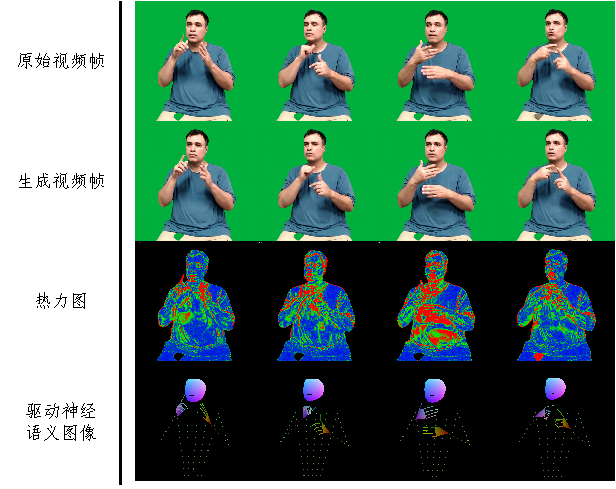
\includegraphics[width=0.9\textwidth]{./m_figures/chapter4/result/how2sign.pdf}
	\caption{How2Sign 生成结果}
	\label{fig:how2sign}
\end{figure}

图~\ref{fig:how2sign}~中展示了本节模型在 How2Sign 半身数据集中人物形象的建模效果。分别绘制了在测试集中原始视频帧、模型生成视频帧、以及带背景掩码的由二者像素差值计算得到的热力图,以及神经语义图像。
根据图中结果分析,本文提出的模型针对半身数字人场景同样能够很好的建模,在该测试集中,模型在手部动作、衣服纹理等方面均取得了较好的效果。尤其针对手部,模型生成的手部在热图虽然显示与原始视频帧存在较大误差,但通过对比原始视频帧和生成视频帧可以发现其情况与 Ted-talk 中类似,生成帧的手部与原始帧视频在视觉上相比具有更高的清晰度。
但因为手语数据集与演讲场景不同,缺少更丰富的面部表情,在该测试集中,模型生成的面部表情较单一,与原始视频帧存在差异,但从数字人整体形象上来看,具有良好的建模效果。

综上所述,本节实验的定性结果与定量结果基本吻合,本文提出的全局人体特征和局部位置特征的融合增强方法很好的与基于人体多特征合成图像融合的基准模型相结合,能够在全身、半身数字人建模任务中都具有良好的效果。证明了当前方案针对数字人建模任务的有效性。

\section{本章小结}

本章提出了基于全局人体特征和局部位置特征的融合增强方案。在本章中,详细介绍了基于 StyleUNet 的多维度特征融合数字人建模模型架构,该架构兼顾了模型生成的质量与生成速度,同时能够很好的利用上一章节构建的细粒度多维度合成图像,达到良好的可控性。同时通过在基础架构上分别添加双段时序编码、局部位置多判别器和基于大模型的人体特征损失设计解决了潜在的闪烁伪影问题,并进一步提高了数字人图像的生成质量。

在实验部分本章对比测评了不同时序编码方案和不同规模的大模型全局人体特征引导效果,通过消融实验进一步验证了各模块设计的有效性,并被基于全局人体特征和局部位置特征融合增强的模型作为基础模型。最后本章进一步通过多场景测评,通过在不同数据集多个场景和人物上进行了性能测评,证明了本文的基础方案针对多种数字人建模场景均具有可观的生成质量。

在下一章节的实验中,模型将进一步与现有开源的先进模型进行横向对比,证明本文模型所具有的实时性与生成质量优势。